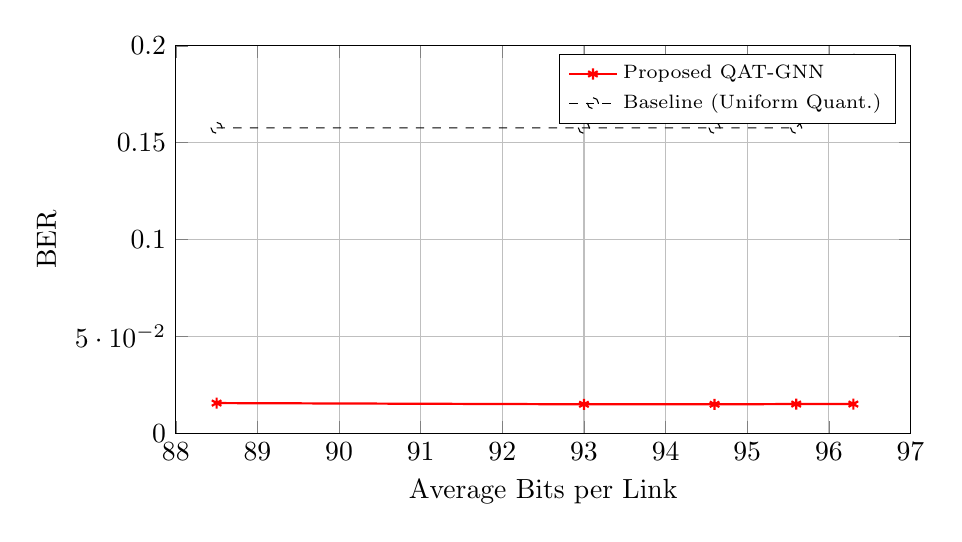
\begin{tikzpicture}
\begin{axis}[
    width=0.9\linewidth,
    height=6.5cm,
    xlabel={Average Bits per Link},
    ylabel={BER},
    xmin=88, xmax=97,
    ymin=0, ymax=0.2,
    grid=both,
    legend style={at={(0.98,0.98)},anchor=north east,font=\scriptsize},
    legend cell align={left}
]
\addplot[color=red,mark=asterisk,thick] coordinates {
(88.5, 0.01550) (93.0, 0.01487) (94.6, 0.01487) (95.6, 0.01500) (96.3, 0.01500)
};
\addlegendentry{Proposed QAT-GNN}

\addplot[color=black,mark=o,dashed] coordinates {
(88.5, 0.15762) (93.0, 0.15762) (94.6, 0.15762) (95.6, 0.15762) (96.3, 0.19287)
};
\addlegendentry{Baseline (Uniform Quant.)}
\end{axis}
\end{tikzpicture}